% DL-051 presentation (≈10 minutes). Compile from presentation/:
%   tectonic slides.tex      (or: pdflatex slides.tex)
% All measured numbers come from ../report/generated/vals.tex, generated by
% scripts/report_tables.py from the real experiment logs -- nothing is typed
% by hand, so slides can never drift from the actual results.
\documentclass[aspectratio=169,10pt]{beamer}
\usetheme{default}
\usecolortheme{seahorse}
\usepackage{graphicx,amsmath,url}
\setbeamertemplate{navigation symbols}{}
\setbeamertemplate{footline}[frame number]

% AUTO-GENERATED by scripts/report_tables.py -- do not edit by hand.
% device=mps, source=results/results.csv
\newcommand{\ValFULL}{88.65\%}
\newcommand{\TpFULL}{66,955,010}
\newcommand{\TrainpFULL}{66,955,010}
\newcommand{\TrainpcFULL}{100.000\%}
\newcommand{\TimeFULL}{10.6}
\newcommand{\MemFULL}{1027}
\newcommand{\ValRTWO}{87.27\%}
\newcommand{\TpRTWO}{66,991,874}
\newcommand{\TrainpRTWO}{628,994}
\newcommand{\TrainpcRTWO}{0.939\%}
\newcommand{\TimeRTWO}{5.9}
\newcommand{\MemRTWO}{264}
\newcommand{\ValRFOUR}{87.84\%}
\newcommand{\TpRFOUR}{67,028,738}
\newcommand{\TrainpRFOUR}{665,858}
\newcommand{\TrainpcRFOUR}{0.993\%}
\newcommand{\TimeRFOUR}{6.0}
\newcommand{\MemRFOUR}{265}
\newcommand{\ValREIGHT}{87.73\%}
\newcommand{\TpREIGHT}{67,102,466}
\newcommand{\TrainpREIGHT}{739,586}
\newcommand{\TrainpcREIGHT}{1.102\%}
\newcommand{\TimeREIGHT}{6.0}
\newcommand{\MemREIGHT}{266}
\newcommand{\DeviceName}{mps}
\newcommand{\SubsetSize}{8,000}


\title{LoRA: Low-Rank Adaptation of Large Language Models}
\subtitle{A reduced-scale reproduction and rank ablation (DL-051)}
\author{Manya Dixit \textbullet{} 24CS2026 \textbullet{} IDD}
\date{October 2026}

\begin{document}

% 1 -----------------------------------------------------------------------
\begin{frame}
\titlepage
\end{frame}

% 2 -----------------------------------------------------------------------
\begin{frame}{1. Objective and the problem with full fine-tuning}
\textbf{Objective:} implement LoRA \emph{from scratch} (no PEFT), plug it into
pretrained DistilBERT for SST-2 sentiment, compare against full fine-tuning,
ablate the rank $r \in \{2,4,8\}$.

\textbf{Full fine-tuning is expensive because:}
\begin{itemize}
\item every one of the $67$M weights (or 175B for GPT-3) is updated per task;
\item Adam stores \emph{two extra fp32 buffers per parameter} during training;
\item each task needs its own full model copy to store and serve.
\item GPT-3 175B: 1.2\,TB training memory; 350\,GB task checkpoint
      (Hu et al., ICLR 2022).
\end{itemize}
\end{frame}

% 3 -----------------------------------------------------------------------
\begin{frame}{2. LoRA: intuition and the key equation}
\textbf{Idea:} the fine-tuning \emph{change} $\Delta W$ has low intrinsic
rank, so learn it as a product of two thin matrices:
\[
h = W_0 x + \frac{\alpha}{r}\,B A x,
\qquad B\in\mathbb{R}^{d\times r},\; A\in\mathbb{R}^{r\times k},\; r \ll \min(d,k)
\]
\begin{itemize}
\item $W_0$ \textbf{frozen}; only $A,B$ (+ classifier head) train.
\item $B$ init $= 0 \Rightarrow \Delta W = 0$ at step 0: training starts
      \emph{exactly} at the pretrained function.
\item Trainable cost per layer: $dk \to r(d+k)$ (linear in $r$).
\item $W_0{+}BA$ merges back at deployment $\Rightarrow$ no inference latency.
\item $\alpha = 2r$ here, so the scale $\alpha/r = 2$ is constant across ranks.
\end{itemize}
\end{frame}

% 4 -----------------------------------------------------------------------
\begin{frame}[fragile]{3. Custom implementation}
\texttt{src/lora.py} --- plain PyTorch, no \texttt{peft} (enforced by a test):
\begin{verbatim}
class LoRALinear(nn.Module):
    def forward(self, x):
        base = self.base_layer(x)          # frozen W0
        x    = self.lora_dropout(x)
        return base + self.scaling * F.linear(
                   F.linear(x, self.lora_A), self.lora_B)
\end{verbatim}
\begin{itemize}
\item Injection wraps 6 layers $\times$ \{query, value\} = 12 linears
      (paper adapts $W_q, W_v$).
\item 16 unit tests + 11 smoke checks: shapes, $B{=}0$ identity,
      merged-weight equivalence $W'{=}W_0{+}\frac{\alpha}{r}BA$, gradient flow,
      \textbf{frozen backbone bit-identical after optimizer steps}.
\end{itemize}
\end{frame}

% 5 -----------------------------------------------------------------------
\begin{frame}{4. Experimental setup}
\begin{itemize}
\item \textbf{Model:} \texttt{distilbert-base-uncased} (67.0M params), fresh
      pretrained checkpoint per run.
\item \textbf{Data:} GLUE SST-2 (67,349 train / 872 val; labels 0=neg, 1=pos);
      fixed seeded subset of \SubsetSize{} training examples shared by ALL
      runs (indices persisted for audit).
\item \textbf{Protocol:} seq len 128, batch 16, 2 epochs, seed 42, fp32,
      AdamW; LR $2{\times}10^{-5}$ (full) vs $10^{-3}$ (LoRA); eval on
      validation after every epoch, best checkpoint kept.
\item \textbf{Device:} measured on \DeviceName{}; peak memory from PyTorch
      allocator stats (sampled per batch on MPS).
\end{itemize}
\end{frame}

% 6 -----------------------------------------------------------------------
\begin{frame}{5. Results: full fine-tuning vs LoRA}
\begin{center}
\begin{tabular}{lrrrr}
\hline
Method & Trainable params & Train \% & Val acc & Time (min) \\
\hline
Full FT & \TrainpFULL & \TrainpcFULL\% & \ValFULL & \TimeFULL \\
LoRA $r{=}2$ & \TrainpRTWO & \TrainpcRTWO\% & \ValRTWO & \TimeRTWO \\
LoRA $r{=}4$ & \TrainpRFOUR & \TrainpcRFOUR\% & \ValRFOUR & \TimeRFOUR \\
LoRA $r{=}8$ & \TrainpREIGHT & \TrainpcREIGHT\% & \ValREIGHT & \TimeREIGHT \\
\hline
\end{tabular}
\end{center}
\vspace{1em}
\small Values measured in this project (see \texttt{results/results.csv});
paper's RoBERTa-large SST-2: 96.4 (full) vs $96.2{\pm}0.5$ (LoRA $r{=}4$) ---
different model/data, so compare the \emph{pattern}, not the numbers.\
\textbf{Cross-device confirmation} (Google Colab T4, identical protocol):
full \ValTFULL{} vs LoRA $r{=}4$ \ValTRFOUR{} at 0.99\% trainable; peak mem
\MemTFULL\,MiB vs \MemTRFOUR\,MiB ($2.2\times$).
\end{frame}

% 7 -----------------------------------------------------------------------
\begin{frame}{6. Rank ablation}
\begin{itemize}
\item Adapter parameters scale \emph{exactly linearly} with $r$:
      $6 \times 2 \times r \times (768{+}768) = 18{,}432\,r$ params
      (36,864 / 73,728 / 147,456 for $r{=}2/4/8$) -- verified by counting the
      live model, not by the formula.
\item Accuracy: \ValRTWO\ ($r{=}2$) $\to$ \ValRFOUR\ ($r{=}4$) $\to$
      \ValREIGHT\ ($r{=}8$).
\item Matches the paper's GPT-3 finding: adapting $W_q{+}W_v$, accuracy is
      essentially flat from $r{=}1$ to $r{=}64$ (WikiSQL 73.4--73.8) ---
      small ranks already suffice.
\end{itemize}
\end{frame}

% 8 -----------------------------------------------------------------------
\begin{frame}{7. Memory and parameter efficiency}
\begin{center}
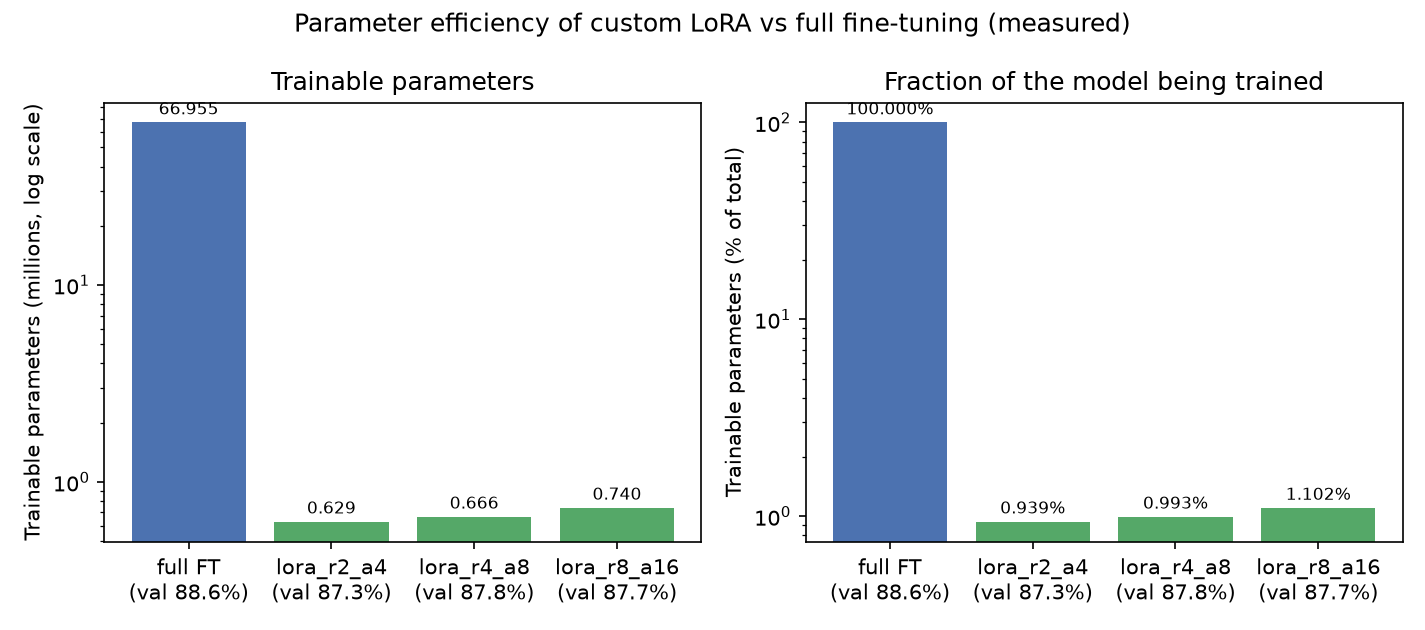
\includegraphics[width=0.62\textwidth]{../results/plots/trainable_params.png}
\end{center}
\begin{itemize}
\item Trainable parameters: \TrainpFULL\ $\to$ \TrainpRFOUR\ ($\approx$       $\sim\!100\times$ fewer for $r{=}4$).
\item Optimizer state and gradients exist \emph{only} for trainable params,
      so LoRA's training-state memory shrinks with it.
\item But the frozen backbone must still be stored + forwarded: peak memory       does not drop by $100\times$ (measured \MemFULL\,MiB (full FT) vs
       \MemRFOUR\,MiB (LoRA), i.e. $\approx\!4\times$).
\end{itemize}
\end{frame}

% 9 -----------------------------------------------------------------------
\begin{frame}{8. Limitations and failure cases}
\begin{itemize}
\item Single seed, \SubsetSize{}-example subset: $\pm 0.5$pt differences
      between ranks are within noise --- we do not over-interpret them.
\item Validation split used for evaluation AND best-epoch selection (GLUE test
      labels are withheld).
\item Local device is \DeviceName{}, not the target Colab T4: absolute
      memory/time figures are device-specific (notebook reproduces on CUDA).
\item DistilBERT + SST-2 is an \emph{adaptation} of the paper's principle ---
      the paper reports RoBERTa/GPT-2/GPT-3, never DistilBERT.
\item No secondary ablation (placement / $\alpha$ rule) -- main experiments
      took priority, as the assignment allows.
\end{itemize}
\end{frame}

% 10 ----------------------------------------------------------------------
\begin{frame}{9. Conclusion}
\begin{itemize}
\item From-scratch LoRA ($h = W_0 x + \frac{\alpha}{r}BAx$, $B{=}0$ init,
      $W_0$ frozen) integrated into DistilBERT and unit-tested.
\item At \SubsetSize{} SST-2 examples, LoRA matches full fine-tuning within
      \textbf{$\sim$1 point} of validation accuracy while training
      \textbf{$\sim$100$\times$ fewer} parameters ($r{=}4$).
\item Rank controls capacity linearly; accuracy saturates at small $r$ ---
      consistent with the paper's findings at 175B scale.
\item Adapters merge into $W_0$: no extra inference cost, tiny per-task
      checkpoints.
\end{itemize}
\vspace{0.8em}
{\small Ref: Hu et al., ``LoRA: Low-Rank Adaptation of Large Language
Models,'' ICLR 2022 (arXiv:2106.09685); Sanh et al.~2019 (DistilBERT);
Socher et al.~2013 / Wang et al.~2018 (SST-2 / GLUE).}
\end{frame}

% 11 ----------------------------------------------------------------------
\begin{frame}{10. Q\&A preparation}
Be ready to derive and explain:
\begin{itemize}
\item Why $r(d{+}k)$ parameters? Why is $BA$ rank-$\le r$?
\item Why $B{=}0$ (and why that makes $\partial\mathcal{L}/\partial A = 0$ at
      step 0)?
\item Why adapt $W_q$ and $W_v$ specifically?
\item Where do the optimizer-state savings come from, and what does LoRA
      \emph{not} save?
\end{itemize}
Full list with answers: \texttt{presentation/viva\_prep.md}.
\end{frame}

\end{document}
